\section{Durchführung}
Bei diesem Experiment werden vier Messungen durchgeführt. 

Zunächst wird die Leerlaufspannung einer Monozelle unmittelbar mit
einem Spannungsmesser ermittelt. Der Eingangswiderstand $R_v$ wird 
dabei notiert. 

Danach wird die Klemmspannung $U_k$ in Abhängigkeit vom Belastungsstrom
$I$ gemessen. Dazu wird der Aufbau gemäß Abbildung \ref{fig:Messschaltung} verwendet. Der 
Belastungswiderstand $R_a$ wird in einem Bereich von 0 - 50\si{\ohm} 
variiert. Dabei werden 14 Messwerte für $U_k$ und $I$ notiert.

\begin{figure}[H]
\center
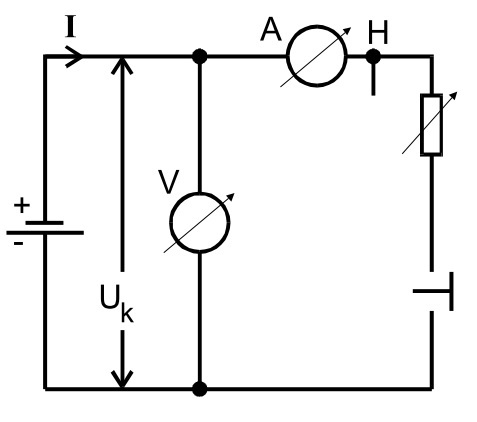
\includegraphics[scale=0.3]{Aufbau_b.jpg}
\caption{Messschaltung zur Bestimmung von $U_0$ und $R_i$}
\label{fig:Messschaltung}
\end{figure}

Im nächsten Schritt wird eine Gegenspannung an die Monozelle gemäß Abbildung
\ref{fig:Messschaltung2} angelegt. Diese ist zirka 2V größer als die Leerlaufspannung
$U_0$. Durch die Gegenspannung fließt ein Strom in entgegengesetzter Richtung durch die 
Schaltung. Wie zuvor wird $U_k$ in Abhängigkeit von $I$ gemessen. 

\begin{figure}
\center
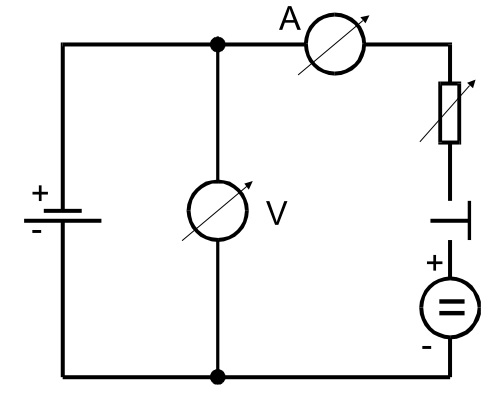
\includegraphics[scale=0.3]{Aufbau_c.jpg}
\caption{Verwendung einer Gegenspannung}
\label{fig:Messschaltung2}
\end{figure}

Bei der letzten Messung benutzt man einen Aufbau gemäß Abbildung \ref{fig:Messschaltung}.
Statt einer Monozelle als Spannungsquelle wird allerdings der Sinus- und 
Rechteckausgang eines RC - Generators verwendet. 
Für jeden Ausgang werden jeweils 11 und 17 Messwerte notiert. Bei der 
Rechteckspannung liegt der Variationsbereich von $R_a$ bei 20 - 250\si{\ohm} 
und bei der Sinusspannung bei 0.1 - \SI{5}{\kilo\ohm}.
Zu beachten ist, dass die Eichungen der Messgeräte nur für einen bestimmten 
Frequenzbereich gültig sind. Deswegen wird die Frequenz der Spannungen auf
einen Wert in diesem Bereich festgelegt.

\label{sec:Durchführung}
